%-----------------------------------------------------------------------
%
% File Name: thesis.tex
%
% Author: Kelley, D. B.
%
% Revision: $Id$
%
%-----------------------------------------------------------------------

% document class and packages
\documentclass[12pt,notitlepage]{report}
\usepackage{bibunits}
\usepackage{suthesis}
\usepackage{graphicx}
\usepackage{color}
\usepackage{amsmath}
\usepackage{amssymb}
\usepackage{amsfonts}
\usepackage[bookmarksnumbered, bookmarksopen, breaklinks, colorlinks, linkcolor=blue, citecolor=magenta]{hyperref}

%\usepackage{caption}
%\usepackage{rotating}
%\usepackage{tensor}

\pdfoutput=1
\DeclareGraphicsExtensions{.pdf,.png}

\hbadness=10000

% new command definitions
\newcommand{\half}{\frac{1}{2}}
\newcommand{\ospsd}{\ensuremath{S_n\left(\left|f_{k}\right|\right)}}

% journal definitions
\newcommand{\apj}{{\it Astrophysical J.}}
\newcommand{\apjl}{{\it Astrophysical J.}}
\newcommand{\aap}{{\it Astron. and Astrophys.}}
\newcommand{\cmp}{{\it Commun. Math. Phys.}}
\newcommand{\grg}{{\it Gen. Rel. Grav.}}
\newcommand{\cqg}{{\it Class. Quant. Grav.}}
\newcommand{\lr}{{\it Living Reviews in Relativity}}
\newcommand{\mnras}{{\it Mon. Not. Roy. Astr. Soc.}}
\newcommand{\pr}{{\it Phys. Rev.}}
\newcommand{\prl}{{\it Phys. Rev. Lett.}}
\newcommand{\prd}{{\it Phys. Rev. D}}
\newcommand{\pra}{{\it Phys. Rev. A}}
\newcommand{\prsl}{{\it Proc. R. Soc. Lond. A}}
\newcommand{\ptrsl}{{\it Phil. Trans. Roy. Soc. London}}
\newcommand{\rmp}{{\it Rev. Mod. Phys.}}

\newcommand{\tcr}{\textcolor{red}}
\newcommand{\tcb}{\textcolor{blue}}
\newcommand{\tcm}{\textcolor{magenta}}
\newcommand{\tcg}{\textcolor{green}}
\newcommand{\tcp}{\textcolor{purple}}

\begin{document}
\title{Detector Characterization of Advanced LIGO}
\author{Thomas J. Massinger}
\majorprof{Peter R. Saulson}
\previousdegree{}{B.S. Physics, Utica College, Utica, NY 13502}
%\previousdegree{M.S. Syracuse University, Syracuse, NY, 2013}{}
\submitdate{June 2016}
\degree{Doctor of Philosophy}
\program{Physics}
\copyrightyear{2015}
\majordept{Physics}
\havededicationtrue
\dedication{to diglett}
\haveminorfalse
\copyrighttrue
\doctoratetrue
\figurespagetrue
\tablespagetrue

\Abstract{% taken from angular theory paper
Placeholder with reference (Sidles-Sigg instability \cite{Sidles06}).

}

\beforepreface

\prefacesection{Preface}
The work presented in this thesis stems from my participation in the LIGO
Scientific Collaboration (LSC). This work does not reflect the
scientific opinion of the LSC and it was not reviewed by the collaboration.



%\vspace*{0.5cm}
%
%\noindent Chapter \ref{ch:photothermal} is based on material from
%
%\vspace*{0.25cm}
%
%\noindent David B. Kelley~{\it et~al.}, ``Observation of photo-thermal feed-back in a stable dual-carrier optical spring,''  to be submitted to
%\prd.
%
%\vspace*{0.25cm}
%
%\noindent Chapter \ref{ch:angular} is based on 
%
%\vspace*{0.25cm}
%
%\noindent David B. Kelley~{\it et~al.}, ``Angular Trap Demonstration,'' to be submitted to
%\prd

\prefacesection{Acknowledgments}
I would like to thank many people for all the wonderful things they have done over the past 3000 years or so.



\afterpreface

\Chapter{Introduction}
\label{ch:introduction}
% $Id$

In chapter \ref{c:findchirp} we describe in detail the algorithms used to
inspiral signals from binary neutron starts and binary black hole MACHOs in
the LIGO data.  findchirp. We first carefully define the conventions that we
use for analysis quantities in section \ref{s:conventions}; in particular the
definition of the Fourier transform and the power spectral density. Section
\ref{s:waveforms} gives a brief description of the the waveforms used and
section \ref{s:matchedfilter} describes the implementation of the matched
filter.  Spurious noise may cause the output of the matched filter to be large
and so in section \ref{s:chisq} we describe our implementation of the $\chi^2$
time--frequency discriminator proposed in~\cite{allen}. Section
\ref{s:practical} contains additional details of the search particular to our
implementation: the computation of the inverse power spectrum and the trigger
selection algorithm. This is followed by a brief conclusion which summarized
the methods used and outlines some future directions for improvement.

\section{Fourier Transform Conventions}
\label{s:ftconv}

There are two possible sign conventions for the Fourier transform of a time
domain quantity $v(t)$. In this thesis, we define the Fourier transform
$\tilde{v}(f)$ of a $v(t)$ to be
\begin{equation}
\label{eq:ft}
\tilde{v}(f)=\int_{-\infty}^\infty dt\,v(t)\, e^{- 2 \pi i f t}
\end{equation}
and the inverse Fourier transform to be 
\begin{equation}
\label{eq:ift}
v(t)=\int_{-\infty}^\infty df\,\tilde{v}(f)\, e^{2 \pi i f t}.
\end{equation}
This convention differs from that used in some gravitational wave literature,
but is the adopted convention in the LIGO Scientific Collaboration.

%\Chapter{Conclusion}
%\label{ch:conclusion}
%\section{Summary}

aLIGO has begun taking data and will achieve design sensitivity over the next few years. At that point, the next generation of upgrades and improvements must be nearly ready to implement. One possible such upgrade would be to damp the unwanted angular motion in the test masses using radiation pressure feedback. This has the potential benefits of reducing the angular noise of the system and thus also reducing the amount of noise that couples from angular motion into cavity length.  
 
We have explored the implementation and uses of radiation pressure feedback, optical springs, to control the motion of a mirror. 
We demonstrated in several ways the underlying principles and behavior of optical springs, in both straight and folded cavities.
We discussed the mechanical design of the experiment, with the addition of blade springs to reduce the influence of seismic noise on the experiment.
We reviewed the feedback and controls in use for the optical traps. 
We measured and modeled the causes and effects of the photothermal effect in an optical spring system.
We explored one- and two-degree-of-freedom traps, and, while we could not get the angular trap stably locked for more than two seconds, we have laid out the path to do so.
We designed and modeled a full-scale implementation of angular optical springs to damp the Sidles-Sigg instability in the aLIGO configuration.

These developments should lay a strong groundwork for continued research into the applications and uses of radiation pressure feedback in aLIGO and beyond.

\section{Future work}

There are several things left unfinished that will hopefully deliver interesting results:

\begin{enumerate}
	\item Improving the stability  of the SU angular optical trap experiment and damping the 66 Hz resonance that seems to be preventing extended locks.
	There are a number of possibilities to increase the bandwidth and damp the motion outlined in Section \ref{sec:bandwidth}.
	\item Exploring the possibility of a a single stable optical spring with a specialized optical coating.
	We expect that dielectric coating manufacturers could do a custom run with a very thick first layer to create a ``self-locking'' cavity. The mirror could be mounted using the same cold weld method described in Section \ref{sec:endMirror}, then tested with the single-mirror input coupler from Chapter \ref{ch:photothermal}. 
	\item Designing and demonstrating a large scale angular trap in aLIGO.
	A detailed noise budget needs to be drafted using a modified version of GWINC or a similar tool to insure that we would not be introducing too much thermal noise.
	After that, a prototype of the design would need to be built at e.g. the Caltech 40 m interferometer to develop control systems and test predictions.
\end{enumerate}

%For each bullet, add at lease one more sentence that discusses how you would go about these items.
%What is the first thing to be done? What hardware needs to be purchased, changed? Etc.


%% $Id$
%
%Although the upper limit that we have placed on the rate of binary black hole
%MACHO inspirals in the galaxy is lower than the upper bound of the predicted
%rates, the LIGO interferometers were not at design sensitivity when the S2
%data was taken. At present, the sensitivities of the instruments are
%significantly better than during S2, as can be seen from
%figure~\ref{f:s3strain}, and progress on reducing noise in the interferometers
%continues apace.  The increase in detector sensitivity makes a larger volume
%of the Universe accessible to searches for binary inspirals. In addition to
%this, the amount of data is also increasing as the interferometers become more
%stable.
%
%These improvements in the instruments will increase the chance of detecting
%gravitational waves from binary inspirals. If the rates of binary black hole
%MACHO coalescence are truly as high as predicted, then initial LIGO would
%stand an excellent chance of detecting an inspiral. The first detection of
%gravitational waves will be a major scientific breakthrough and will yield and
%enormous amount of scientific information, particularly if the detection came
%from a binary black hole MACHO. The length of binary black hole MACHO
%inspirals in the sensitive band of the interferometer will allow extremely
%accurate parameter estimation as well as tests of post-Newtonian theory. For
%systems with total mass greater than $\sim 0.64\,\mathrm{M}_\odot$ LIGO will
%be sensitive to the coalescence of the binary and will be able to study the
%strong gravitational field effects when two binary black holes merge. When
%this is coupled with the accurate parameter estimation available from the
%earlier part of the waveform, the inspiral of a binary black hole MACHO could
%be an excellent laboratory for General Relativity.  A detection would also
%impact the studies of halo dark matter and early universe physics, providing a
%MACHO component to the halo and suggesting that primordial black holes do
%indeed form in the universe.
%
%In the absence of detection, the improvements in detector sensitivity will
%dramatically improve the upper limits placed on the rate of binary black hole
%MACHO inspirals. Once these rates are below the predicted rates, we may begin
%to use observations from gravitational wave interferometers to constrain the
%fraction of galactic halos in the form of primordial black hole MACHOs. While
%this may not be as significant as a detection, it will still be of interest to
%the astrophysical community.
%
%\newpage 
%
%\begin{figure}[p]
%\vspace{5pt}
%\begin{center}
%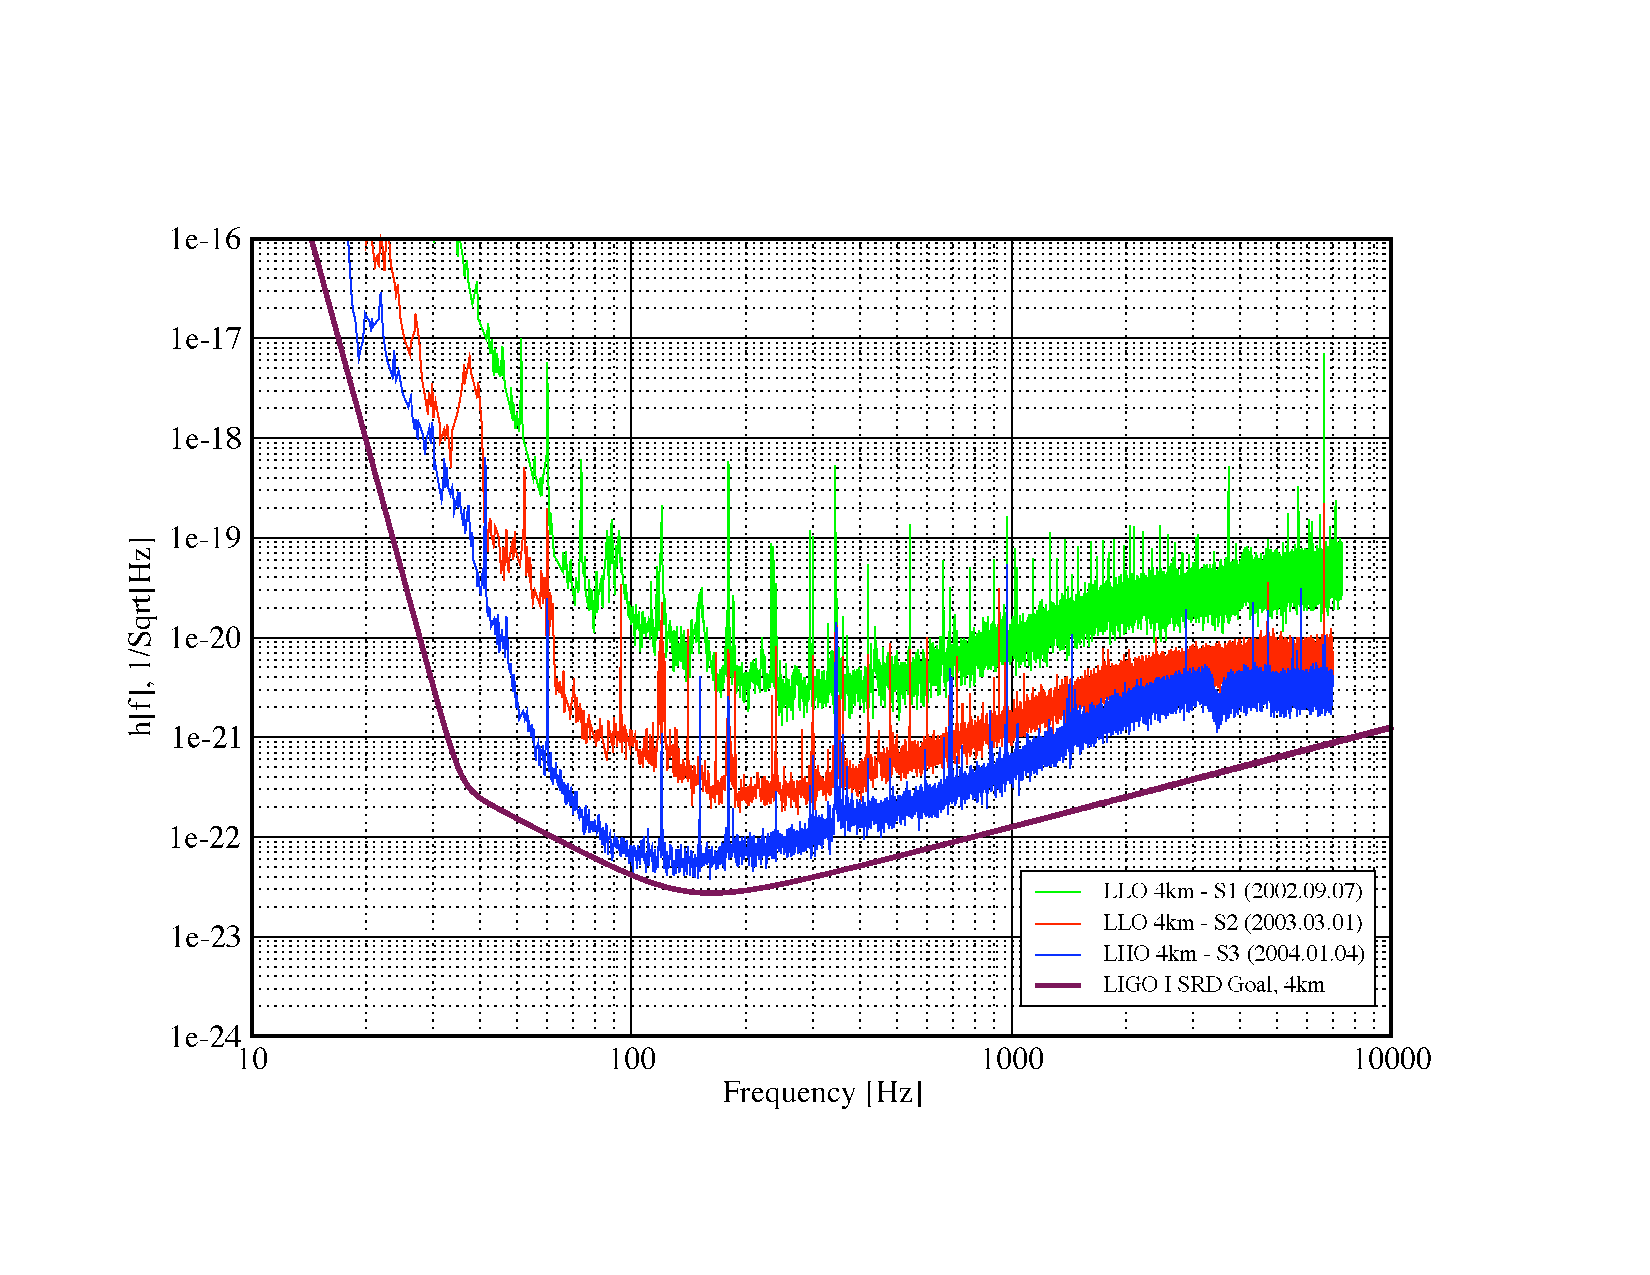
\includegraphics[width=\textwidth]{figures/conclusion/s3strain}
%\end{center}
%\caption[Comparison of Best LIGO Interferometer Sensitivity]{%
%\label{f:s3strain}
%Comparison of the best sensitivities of the LIGO interferometers between
%science runs. The solid curve shows the design sensitivity for the $4$~km
%interferometers: the LHO $4$~km is only a factor of $\sim 2$ away from design
%at $100$~Hz during S3.
%}
%\end{figure}
%


%\appendix
%\Chapter{Beam Separation}
%\label{ap:beamseparation}
%%\documentclass[12pt]{article}
%\usepackage{fullpage,graphicx}
%\title{Beam seperation}
%\author{David Kelley}
%\begin{document}
%\maketitle

\section{Definitions}
\begin{itemize}
\item $P_m$ Input power of the main beam 
\item $P_s$ Input power of the side beam
\item $f_m$ Main cavity finesse
\item $f_s$ Side cavity finesse
\item $R_c$ Radius of curvature of payload mirror (5 cm)
\item $\theta_m$ Main beam angle from optical axis.  Origin is at center of curvature.
\item $\theta_s$ Side beam angle from optical axis.  Origin is at center of curvature.
\item $c$ Speed of light
\item $R$ Payload mirror radius
\item $h$ Payload mirror thickness
\item $m$ Payload mirror mass
\item $I = \frac{m}{12}(3R^2+h^2)$ Payload mirror moment of inertia
\item $G = \frac{P_mf_m}{P_sf_s}$ Handy constant
\item $d = \theta_mR_c - \theta_sR_c$ Beam spot seperation
\end{itemize}


\newpage
\section{Balancing torques}
We want the mirror to be stationary, so the net torque on the mirror should be zero.

Force on payload mirror due to radiation pressure of the two beams:

$$ F_m = \frac{2P_mf_m}{c} \hspace{20 pt} F_s = \frac{2P_sf_s}{c}$$

$$\tau = F_m\theta_mR_c+F_s\theta_sR_c = 0$$

substituting in $d$,

$$\theta_m = \frac{d}{R_c(1+G)}$$

\section{Eliminating beam coupling}

We propose that there is a spot somewhere on the surface of the payload mirror where the sum of torque and force due to one beam makes the net force zero.  We place one beam spot at $r_1$.  We'd like to put the other beam in the null spot $r_2$ so that there is no force coupling between the two.  

$$Fs=\frac{2P_sf_s}{c} = m\omega^2x \hspace{20pt} x = \frac{F_s}{m\omega^2}$$ 
$$\tau_s = F_sr_1=I\omega^2\phi \hspace{20pt} \phi = \frac{F_s r_1}{I\omega^2}$$

Let's find a point these effects cancel:

$$r_2\phi-x=0 \hspace{20 pt} r_2=\frac{x}{\phi}=\frac{I}{mr_1}$$

It should be noted that the previously used $d$ can also be expressed as $d =r_2-r_1$.

$$r_2 = \theta_2R_c = \theta_mR_c$$

$$r_2 = \frac{d}{1+G}$$

$$\frac{I}{m} = \frac{(r_2-r_1)r_1}{1+G} = \frac{\left(\frac{I}{mr_1}+r_1\right)r_1}{1+G}$$

$$r_1 = \sqrt{\frac{I}{mG}} \hspace{20pt} r_2 = \sqrt{\frac{IG}{m}}$$

These radii are the ideal horizontal distances from the payload mirror optical axis to the beam spots.
%A MATLAB script that computes this seperation is included in this directory, named cavityAngles.m. 



%\end{document}

\clearpage
\bibliographystyle{unsrt}
\bibliography{references}

\addcontentsline{toc}{chapter}{\numberline {Bibliography}}

\clearpage
\birthplacedate{Rochester, NY \>\>July 22, 1989}
\collegewherewhen{%
\>Utica College \>\>2007--2011, \>B.S.\\
\>\su	\>\>2011--2016, \>Ph.D.}

\newpage
\null\vskip1in%
\begin{center}
{\Large\bf Curriculum Vitae}
\end{center}
\vskip 2em
\begin{tabbing}
\tabset
Title of Dissertation\\
\>Detector Characterization of Advanced LIGO
\end{tabbing}
\vskip 1em

\begin{startvita}
\end{startvita}

\renewenvironment{thebibliography}[1]%
  {\begin{list}{\labelenumi\hss}%
     {\usecounter{enumi}\setlength{\labelwidth}{3em}%
      \setlength{\leftmargin}{5em}}}%
  {\end{list}}
\renewcommand{\bibitem}[1]{\item\label{#1}\relax}%
\renewcommand{\theenumi}{\arabic{enumi}}%
\begin{publications}
\putbib[papers]
\end{publications}


\finishvita
\end{document}
